% There are two otion that can be provided to the uofathesis class
% 1) published - adjusts the declaration to include a statement regarding published materials. This is required if any chapters in your thesis have been published.
% 2) international - include this if you are an international student to exclude the paragraph regarding the Australian Government Research Training Program Scholarship 
\documentclass[published]{uofathesis}

% Any packages should go here
\usepackage{lineno,setspace}
\usepackage{caption}
\usepackage{booktabs}
\usepackage{amsmath,amssymb,amsfonts,amsbsy}
\usepackage{rotating,array,multirow}
\usepackage{textcomp}
\usepackage{afterpage, emptypage}
\usepackage{pdflscape}
\usepackage{graphicx,natbib} 
\usepackage{hyperref}
\usepackage{geometry}
\usepackage{layouts}
\usepackage{pdfpages}

% SET MARGINS
\geometry{outer=20mm,inner=35mm}

% ADD HYPERLINKS TO DOCUMENT BUT MAINTAIN BLACK FONT
\hypersetup{colorlinks=true,allcolors=}

\title{The title of my thesis}
\titlesize{\huge} % recommend using any of \large, \Large, \LARGE, \huge, \HUGE, depening on length of title. 
\author{Samuel Jennings}
\degree{Doctor of Philosophy}
\department{Department of Earth Sciences}
\school{School of Rock}

% PATHS TO FIGURES - add these as needed
\graphicspath{
    {chapter1/figures/}
    {chapter2/figures/}
    }

% Use the includeonly command to work on individual chapters at a time.
% Comment out this command to build the entire document.
% \includeonly{chapter1/body}

\begin{document}
\frontmatter
\maketitle

% Create the following tables
\tableofcontents
\listoftables
\listoffigures

% HDR Declaration
\makedeclaration

% Import the various things
\chapter{Acknowledgements}

\noindent
The \textbackslash noindent command and the underlying \textbackslash vspace command is personal preference here and definitely not required. Just something that I preferred after typing out my acknowledgements.
\vspace{0.5\baselineskip}

\noindent
Aute eu laborum enim nulla excepteur id labore ipsum tempor sit nisi. Sunt quis commodo exercitation voluptate Lorem Lorem magna eu magna eu eu irure est minim. Ipsum voluptate consectetur in nulla tempor est eu. Labore esse in id reprehenderit. Voluptate enim id et dolor labore mollit aliqua nulla reprehenderit reprehenderit incididunt duis aliquip adipisicing.
Qui ex elit laborum laboris ad. Magna nulla do amet proident ad Lorem et eiusmod occaecat quis laboris sint laborum excepteur. Laboris voluptate commodo laboris officia irure dolore deserunt amet reprehenderit mollit sint eu elit. Irure amet dolore nostrud Lorem sint labore quis ad eiusmod aliquip nulla sunt in proident. Irure reprehenderit aliqua minim velit et irure sunt dolor proident occaecat sunt sunt reprehenderit. Laborum ut dolore do culpa ullamco reprehenderit est excepteur pariatur veniam aliquip amet occaecat. Reprehenderit tempor amet nulla velit laborum.
\vspace{0.5\baselineskip}

\noindent
Dolore aliqua nostrud cillum voluptate minim do reprehenderit reprehenderit do. Quis dolor deserunt esse quis tempor. Anim amet eu ipsum officia occaecat officia minim ad voluptate nisi.
Cupidatat reprehenderit irure aliquip in anim aliquip ea. Deserunt sit esse laboris sunt occaecat sunt aute fugiat amet veniam cupidatat do. Ea officia tempor nostrud duis mollit ea sunt sint sint anim do aute laboris. Quis velit laboris sint Lorem eiusmod in nostrud nisi nisi cupidatat nulla. Exercitation quis aliqua ipsum ut laborum velit pariatur irure nulla sint consequat do minim adipisicing.
\vspace{0.5\baselineskip}
\chapter{Abstract}

Here's what it's all about! Labore minim irure occaecat fugiat nulla sint labore et laborum eiusmod. In Lorem voluptate in do do aliqua labore velit nisi velit cupidatat deserunt. Ut aliqua officia magna id sit incididunt nulla. Mollit eu ad aute ullamco deserunt fugiat sint eiusmod aliqua cupidatat. Velit id ut est consequat duis velit. Amet quis proident culpa ea.

Cupidatat enim velit Lorem duis. Eiusmod id laboris anim nulla ad. Exercitation qui anim occaecat quis fugiat. Nisi sit minim fugiat fugiat culpa do aute consequat. Exercitation exercitation non voluptate in labore do. Consectetur sint consectetur id quis mollit.

Eu laboris deserunt dolore quis ut qui qui cupidatat irure. Est sit enim officia labore esse et duis magna incididunt nisi eiusmod officia voluptate. Consequat magna dolore laboris officia dolore. Tempor esse magna commodo ipsum aliqua aliqua commodo do cupidatat veniam velit aliquip dolore ad. Do veniam fugiat dolore aliquip esse ex nisi id cupidatat culpa nisi sit esse. Minim non est anim ad laborum velit commodo eu est. Ad labore occaecat exercitation dolor non dolor id ullamco.

Commodo non velit velit exercitation officia anim officia officia ullamco officia ad. Enim esse adipisicing in deserunt quis voluptate pariatur tempor. Ipsum magna minim ipsum consequat amet minim enim ea. Esse enim do aute commodo occaecat eiusmod quis laborum exercitation consectetur consequat mollit id. Occaecat anim sunt mollit duis non commodo non consequat eu aliquip. Occaecat eu quis minim commodo. Consequat officia velit anim reprehenderit Lorem nulla aute magna culpa magna.

Ipsum Lorem et occaecat ipsum mollit. Excepteur duis laborum amet mollit enim adipisicing ipsum minim aliqua deserunt anim sit dolor. Anim ad incididunt nisi eu.



\mainmatter
\introduction

The introduction environment is specific to the uofa latex class. The reason I created it centers around how the introduction is presented in the Table of Contents. Using this environment, the introduction does not count towards chapters in the thesis and therefore does not receive a preceding number in the TOC. SO why not just include this in the \textbackslash fronmatter declaration? Because I wanted the introduction to count towards page numbering. Notice how the `Introduction' label in the TOC referes to page 1 of the thesis? Compared to `Abstract' which is labelled using roman numerals.
This was something I did as a personal preference. If you don't like it, use \textbackslash section\{Introduction\} instead.

Lorem ipsum dolor sit amet, consectetur adipiscing elit. Fusce gravida mauris quis massa convallis congue. Maecenas tincidunt purus non fringilla volutpat. Nullam tristique, augue eu aliquam faucibus, felis quam ullamcorper dolor, quis mattis risus sapien a lectus. Duis vehicula, lectus nec pharetra laoreet, elit lacus fermentum risus, rhoncus interdum mi sem id nulla. Nulla augue lacus, accumsan eu purus quis, consequat luctus nisi. Nam fringilla metus in nunc feugiat convallis. Nunc in velit leo. Proin lectus turpis, tristique nec finibus sit amet, interdum a erat. Nulla quis nunc auctor, accumsan magna ut, mattis urna. Sed ac feugiat nibh. Cras vestibulum ante eget sodales bibendum. Ut aliquet finibus ante ut tempus. Suspendisse pellentesque pretium efficitur. Etiam maximus consectetur consequat. Sed hendrerit purus sit amet justo pharetra, a vestibulum tortor consequat. Cras at finibus nisl, et pretium justo.

Phasellus et feugiat risus, eget ultrices risus. Nullam commodo porttitor nibh, in lobortis metus luctus nec. Lorem ipsum dolor sit amet, consectetur adipiscing elit. Maecenas pulvinar neque eget vestibulum lacinia. Suspendisse hendrerit lobortis erat, a consequat nisi posuere id. Curabitur dolor dui, posuere quis mauris sed, euismod aliquet lacus. Fusce ultrices accumsan tempor. Etiam nec massa id nisi facilisis efficitur eu ac est. Mauris ullamcorper metus dictum odio viverra, quis tincidunt felis luctus. Mauris pulvinar lacinia nibh, ac lacinia felis porta et.

Nullam nec tristique leo. Nulla vestibulum, lectus sit amet pharetra laoreet, enim metus accumsan dolor, ac venenatis turpis lacus sed purus. Donec mollis enim dapibus urna pellentesque ornare. Fusce porta magna sed accumsan eleifend. Donec dapibus libero sit amet orci malesuada, sed pulvinar dolor consequat. Aliquam egestas tincidunt tincidunt. Curabitur odio orci, luctus nec convallis at, aliquam non odio. Praesent scelerisque nunc id ante consectetur, nec convallis mi aliquet. Cras felis urna, ornare egestas sem at, elementum consectetur quam. Nam vitae auctor arcu. Sed tempor elit in quam vehicula tincidunt. Nulla accumsan ut ligula et iaculis. Nulla ut sapien sit amet elit tincidunt feugiat ac at mauris. Cras mi massa, laoreet sed iaculis nec, euismod et tortor. In consequat tellus eu elit congue, et elementum sapien molestie.

Mauris vulputate neque ac blandit fermentum. Sed ornare ornare ante, quis rhoncus nisl lacinia non. Morbi interdum leo vitae tortor aliquet condimentum. Nam in urna eu ipsum fringilla tristique. Duis interdum, ex in euismod pharetra, eros ipsum commodo mauris, vel blandit quam nisi a leo. Ut ut placerat arcu. Sed sed cursus massa. Cras nisi odio, maximus non turpis ac, finibus consequat dolor. Aenean vitae massa eget lacus aliquet hendrerit. Aenean fermentum mauris sapien. Proin volutpat vehicula ligula at commodo. Quisque eget magna quis augue facilisis iaculis.

Nulla at posuere est. Vivamus posuere facilisis erat et ornare. Phasellus orci leo, mollis id lacinia vel, condimentum non turpis. Morbi ut consectetur diam. Nulla aliquet felis vel rutrum faucibus. Phasellus sed sapien nibh. Praesent eu magna volutpat nulla hendrerit ullamcorper a non lectus. Nam tincidunt eu massa id porttitor. Praesent nec est pharetra, iaculis velit egestas, lacinia tortor. Donec non justo molestie, rutrum sapien et, feugiat velit. Nunc scelerisque sapien quis consectetur efficitur. Phasellus scelerisque congue semper. In lectus dui, molestie vitae malesuada et, euismod sit amet leo. Morbi cursus, nulla in ullamcorper volutpat, ex sem efficitur eros, sit amet pharetra tortor velit sit amet libero.
% \published{statement_of_authorship.jpg}
\chapter{Here is the first chapter about my exciting research \label{ch:numero_uno}}
\begin{abstract}
The abstract environment restricts the size of the heading and prevents numbering. If this environment is used, the abstract will not be included in the TOC. If you want to include it, use \textbackslash section\{abstract\} instead.

Sit tempor ipsum consequat ea. Nisi exercitation culpa cupidatat excepteur proident mollit. Veniam cupidatat esse Lorem laboris veniam consectetur minim ex sint nostrud. Deserunt pariatur tempor exercitation consectetur tempor cillum elit labore velit consequat officia aliquip id dolore.
Eu pariatur enim dolore esse magna consectetur fugiat. Dolor incididunt elit amet laborum nulla consequat deserunt ex qui cillum. Ut anim cupidatat Lorem aliquip nulla dolor ullamco cupidatat ea nostrud velit pariatur Lorem. Est quis incididunt non eiusmod magna fugiat magna veniam labore irure qui. Non consectetur nulla cupidatat laborum mollit id.

Elit adipisicing velit anim et aliqua dolor mollit incididunt adipisicing voluptate dolor voluptate irure est. Ullamco id veniam ipsum ipsum elit dolore ipsum deserunt est cupidatat. Occaecat laboris consectetur laborum officia laboris cupidatat. Aute fugiat culpa esse magna sunt laboris est sit cupidatat sit adipisicing.
Consectetur est esse ut et do ut non ipsum occaecat et do laboris nisi. In deserunt qui commodo et nulla anim nisi amet ea. Aute voluptate laboris sint veniam et ex est occaecat nostrud non. Ea in sint incididunt amet qui nostrud officia dolor enim ut nisi eiusmod. Sunt anim consequat excepteur dolor id do labore dolor officia ad mollit.

Aliqua ullamco ea eu excepteur duis cillum aliquip do in sit ullamco ea est. Lorem reprehenderit voluptate mollit in dolore id occaecat labore. Est voluptate proident cillum ipsum deserunt tempor in. Incididunt proident deserunt sunt labore minim amet sint. Qui cillum non et dolor minim nulla aute nisi Lorem irure.
\end{abstract}

\section{Introduction}
Dolor non officia anim ut dolor anim duis elit ullamco aliquip magna cupidatat. Magna ea ipsum enim laboris labore duis cillum commodo minim. Id anim sint ad et do deserunt ea esse.
Test reference \citep*{Glover1996}.

Minim sint duis sunt adipisicing ad. Occaecat labore in eu ad dolor adipisicing consequat. Do occaecat Lorem consectetur quis aliquip dolore consequat aliquip proident voluptate est ipsum cillum. Dolor ea veniam adipisicing veniam do ut laborum consequat laboris reprehenderit aliquip. Excepteur Lorem dolore amet esse dolor duis adipisicing quis dolore laboris cillum voluptate. In mollit aliquip duis do aute.

Culpa eiusmod irure occaecat sint commodo pariatur nostrud anim id velit pariatur. Eiusmod dolore consequat sint enim dolor aliquip minim sit ullamco non occaecat occaecat. Fugiat exercitation nostrud culpa occaecat fugiat adipisicing enim ut occaecat mollit non pariatur. Sint dolor aliquip velit eu do cupidatat quis. Culpa sint velit ex esse ex.

Fugiat amet sit cillum duis. Eiusmod nisi nulla cillum laborum labore non. Officia incididunt ea elit tempor excepteur mollit eiusmod Lorem ullamco. Do cupidatat sunt nisi pariatur proident enim adipisicing pariatur officia incididunt sunt nostrud reprehenderit in. Est amet excepteur ad laborum cillum laboris Lorem officia id. Voluptate velit aute Lorem ea eiusmod veniam.

Ut laboris aute tempor duis ad irure minim ea pariatur eu est tempor mollit anim. Nulla voluptate voluptate nostrud minim exercitation ex qui excepteur sint amet in veniam. Est minim aliquip consequat aliquip aute ullamco enim et aliquip. Aliquip sunt do aute reprehenderit ullamco occaecat consequat non. Ipsum nostrud in culpa adipisicing consectetur eu ad dolore in sint est id.

\section{Background}
Aliquip voluptate enim anim sunt occaecat nisi quis tempor sint Lorem do dolor magna aliqua. Magna voluptate non esse qui nostrud est laborum cupidatat aliquip officia nisi. Officia in veniam id deserunt tempor elit pariatur aute amet ea labore. Minim cillum commodo do aute et ut commodo aliqua sit in. Pariatur ut commodo quis culpa mollit sint Lorem. Nisi velit velit do non commodo reprehenderit aute dolore ullamco ea qui.
Laboris eiusmod velit reprehenderit aliqua eu laboris ea Lorem occaecat ad et anim officia. In pariatur non ullamco consequat sint elit ullamco consectetur aute anim incididunt qui. Et exercitation ad mollit amet. Ipsum esse nisi aliquip duis excepteur. Laboris esse deserunt voluptate nulla laboris exercitation aliqua.

Nisi ad eu et est magna mollit consequat dolor irure quis commodo ex laborum nostrud. Aliquip non nisi occaecat Lorem quis aliquip quis reprehenderit veniam nisi ad elit mollit. Ut quis quis exercitation enim pariatur ut ut sint tempor labore velit id. Aute veniam ex commodo non laboris. Est occaecat excepteur do excepteur ipsum ad quis.
Et exercitation cupidatat cillum nostrud sit do aliqua quis officia ullamco ullamco aute sunt laboris. Laborum officia do pariatur consectetur ut cillum ut id pariatur excepteur exercitation pariatur laboris consectetur. Aliqua cillum id minim commodo nulla Lorem enim nostrud.

Est commodo laboris ea voluptate consectetur aliqua. Nostrud officia magna proident voluptate labore consequat. Esse tempor est est aliqua dolor sunt sit ea sint. Culpa ipsum cillum enim ipsum in cillum esse consectetur. Nulla mollit sunt sint laborum consectetur commodo reprehenderit cupidatat tempor do minim laborum elit anim. Sit id nisi consequat ipsum nostrud reprehenderit ea voluptate deserunt nulla velit nostrud esse.
Ullamco nisi consequat pariatur nisi dolore cupidatat voluptate voluptate sit velit. Velit sit nulla incididunt est ea nulla. Laboris mollit culpa mollit magna reprehenderit adipisicing ut elit deserunt dolore. Quis consectetur incididunt minim exercitation voluptate veniam. Ut irure fugiat quis eiusmod. Voluptate non quis amet incididunt ipsum. Nostrud officia ut commodo incididunt fugiat reprehenderit sunt enim consectetur qui.

Eu enim ut nulla irure pariatur consequat do id excepteur cillum eiusmod sit culpa aliqua. Amet magna mollit tempor elit minim duis laborum cupidatat consequat quis. Magna deserunt esse veniam consequat cupidatat irure ea nulla sunt est aliqua eu aliqua officia. Anim in proident esse voluptate. Deserunt in tempor amet reprehenderit officia exercitation nulla eu nisi qui commodo ullamco ea.
Ea do excepteur laboris exercitation aliquip et. Cupidatat nulla eiusmod incididunt magna labore ea incididunt tempor mollit incididunt. Nisi cupidatat sint incididunt aliquip excepteur pariatur velit in tempor est sint. Culpa cupidatat velit anim dolore irure.

Commodo aliqua non reprehenderit nulla quis culpa incididunt laboris nisi eiusmod. Laboris eu ut et minim sunt excepteur esse eiusmod amet veniam labore do. Consectetur sunt incididunt ipsum tempor eu. Id labore veniam ut nisi non aliqua occaecat eu eiusmod non fugiat sint. Duis velit fugiat nisi esse nostrud laborum.
Sint non irure mollit excepteur amet aliquip excepteur et mollit id in. Ut ad voluptate deserunt ut. Ex culpa nostrud exercitation pariatur aliqua.

\begin{figure}[tb]
  \centering
  
\includegraphics{cat.jpg}
    \caption[A brief caption for the list of figures in the front matter.]{Here's my very long well though out caption that will be included below the figure. It describes everything you could ever want to know about the figure. Recommended width for portrait images is 155mm.}
  \label{fig:cat}
\end{figure}

\section{Methods}
Magna dolore laboris magna et commodo. Ut aliqua veniam officia do in officia consequat proident eu labore esse aliquip mollit. Veniam elit qui nisi amet est sit anim. Labore pariatur excepteur cillum irure quis. Est minim ad culpa commodo est sint excepteur irure labore ex.
Ea id ullamco quis est sunt officia duis. Voluptate ex laborum nostrud minim non fugiat enim. Et velit in culpa et sunt est anim excepteur eiusmod esse. Eu culpa amet aliqua aliquip dolor officia et veniam commodo.
Eu occaecat laboris voluptate aliqua. Esse Lorem amet occaecat aute adipisicing commodo labore non quis est esse. Nulla deserunt consequat officia cupidatat irure minim amet eu velit est ex ex. Ipsum ipsum dolore consequat veniam cillum sit irure. Ipsum deserunt in laboris tempor non laboris est. In enim officia occaecat magna ad est est esse Lorem officia Lorem minim laboris.

Irure nisi elit qui elit id fugiat consectetur deserunt. Ullamco nostrud cillum esse nisi sunt. Proident commodo minim aliquip amet adipisicing amet cupidatat mollit incididunt nisi do excepteur proident voluptate. Duis incididunt exercitation in veniam irure labore reprehenderit sint occaecat et non.
Reprehenderit mollit veniam laboris labore eu consectetur labore culpa dolor magna ex deserunt. Sit eiusmod et duis veniam nulla do veniam eu enim ex eu minim id. Ut ex proident duis tempor et. Eiusmod dolor occaecat sint ipsum officia non pariatur enim tempor est eiusmod.

Id reprehenderit deserunt laborum mollit ullamco veniam laborum aute ad excepteur sit ullamco duis aliqua. Esse dolore do ex eu elit exercitation adipisicing deserunt irure. Et fugiat fugiat est nisi tempor quis. Dolore dolore officia do consectetur minim minim sunt officia culpa et ex.
\section{Results}
  
  % Model misfit
  \begin{table}[t!]
    \centering
    \caption[My brief table caption]{Here's a much longer caption. You can learn about doing latex tables somewhere else. Try googling it like a normal person!}
      \begin{tabular}{lcccc}
      \toprule
        & A & B & C & D \\
      \midrule
      Result 1 & 0.285 & \textbf{0.269} & 0.286 & 0.336 \\
      Result 2 & 0.284 & 0.268 & \textbf{0.279} & 0.322 \\
      Result 3 & 0.406 & \textbf{0.371} & 0.499 & 0.451 \\
      Result 4 & \textbf{1.115} & 0.576 & 0.820 & 0.640 \\
      \bottomrule
      \end{tabular}%
    \label{tab:misfit}%
  \end{table}%

\section{Discussion}
Occaecat do cillum enim aliqua elit qui nisi aliqua ullamco elit labore. Sit sunt adipisicing labore quis aute pariatur. Nulla reprehenderit ex laborum enim velit officia sint. Officia laborum velit ad fugiat cupidatat cillum consectetur dolor. Aute laborum incididunt dolore pariatur quis ad dolore deserunt elit Lorem velit esse dolore anim.
Laborum magna ea laborum qui cupidatat sint ex pariatur. Nulla laboris pariatur culpa minim est ut culpa fugiat amet exercitation nisi proident id anim. Labore elit voluptate minim labore mollit. Aliqua sit magna deserunt in id pariatur sint consectetur culpa anim labore amet in elit. Qui veniam id cupidatat anim aliqua dolore pariatur. Veniam laborum in excepteur laboris anim dolor pariatur ipsum id.

Ea commodo excepteur duis ea voluptate aliqua consequat et. Reprehenderit in dolore et dolor. Aliquip sunt do elit aliqua nisi Lorem sunt nostrud Lorem veniam irure incididunt ut ullamco. Fugiat enim aliqua consectetur sunt aute id dolore ad consequat adipisicing. Voluptate enim culpa pariatur dolor anim. In commodo officia enim proident est reprehenderit aute fugiat consequat dolore sit aute ad.
Cillum dolor sint laboris duis nisi sunt. In laboris veniam cillum cupidatat laboris laboris exercitation. Consectetur consequat nisi est ipsum duis incididunt ullamco elit sunt cupidatat anim exercitation proident eiusmod. Adipisicing reprehenderit incididunt commodo occaecat nostrud ipsum labore tempor sit nostrud occaecat dolor. Ullamco commodo Lorem labore nisi ullamco cupidatat mollit labore et officia enim. Incididunt ad voluptate cillum aliqua proident duis.

\afterpage{
\begin{landscape}
    \begin{figure}[htp] %I recommend you become familiar with what these letters mean!
        \centering
        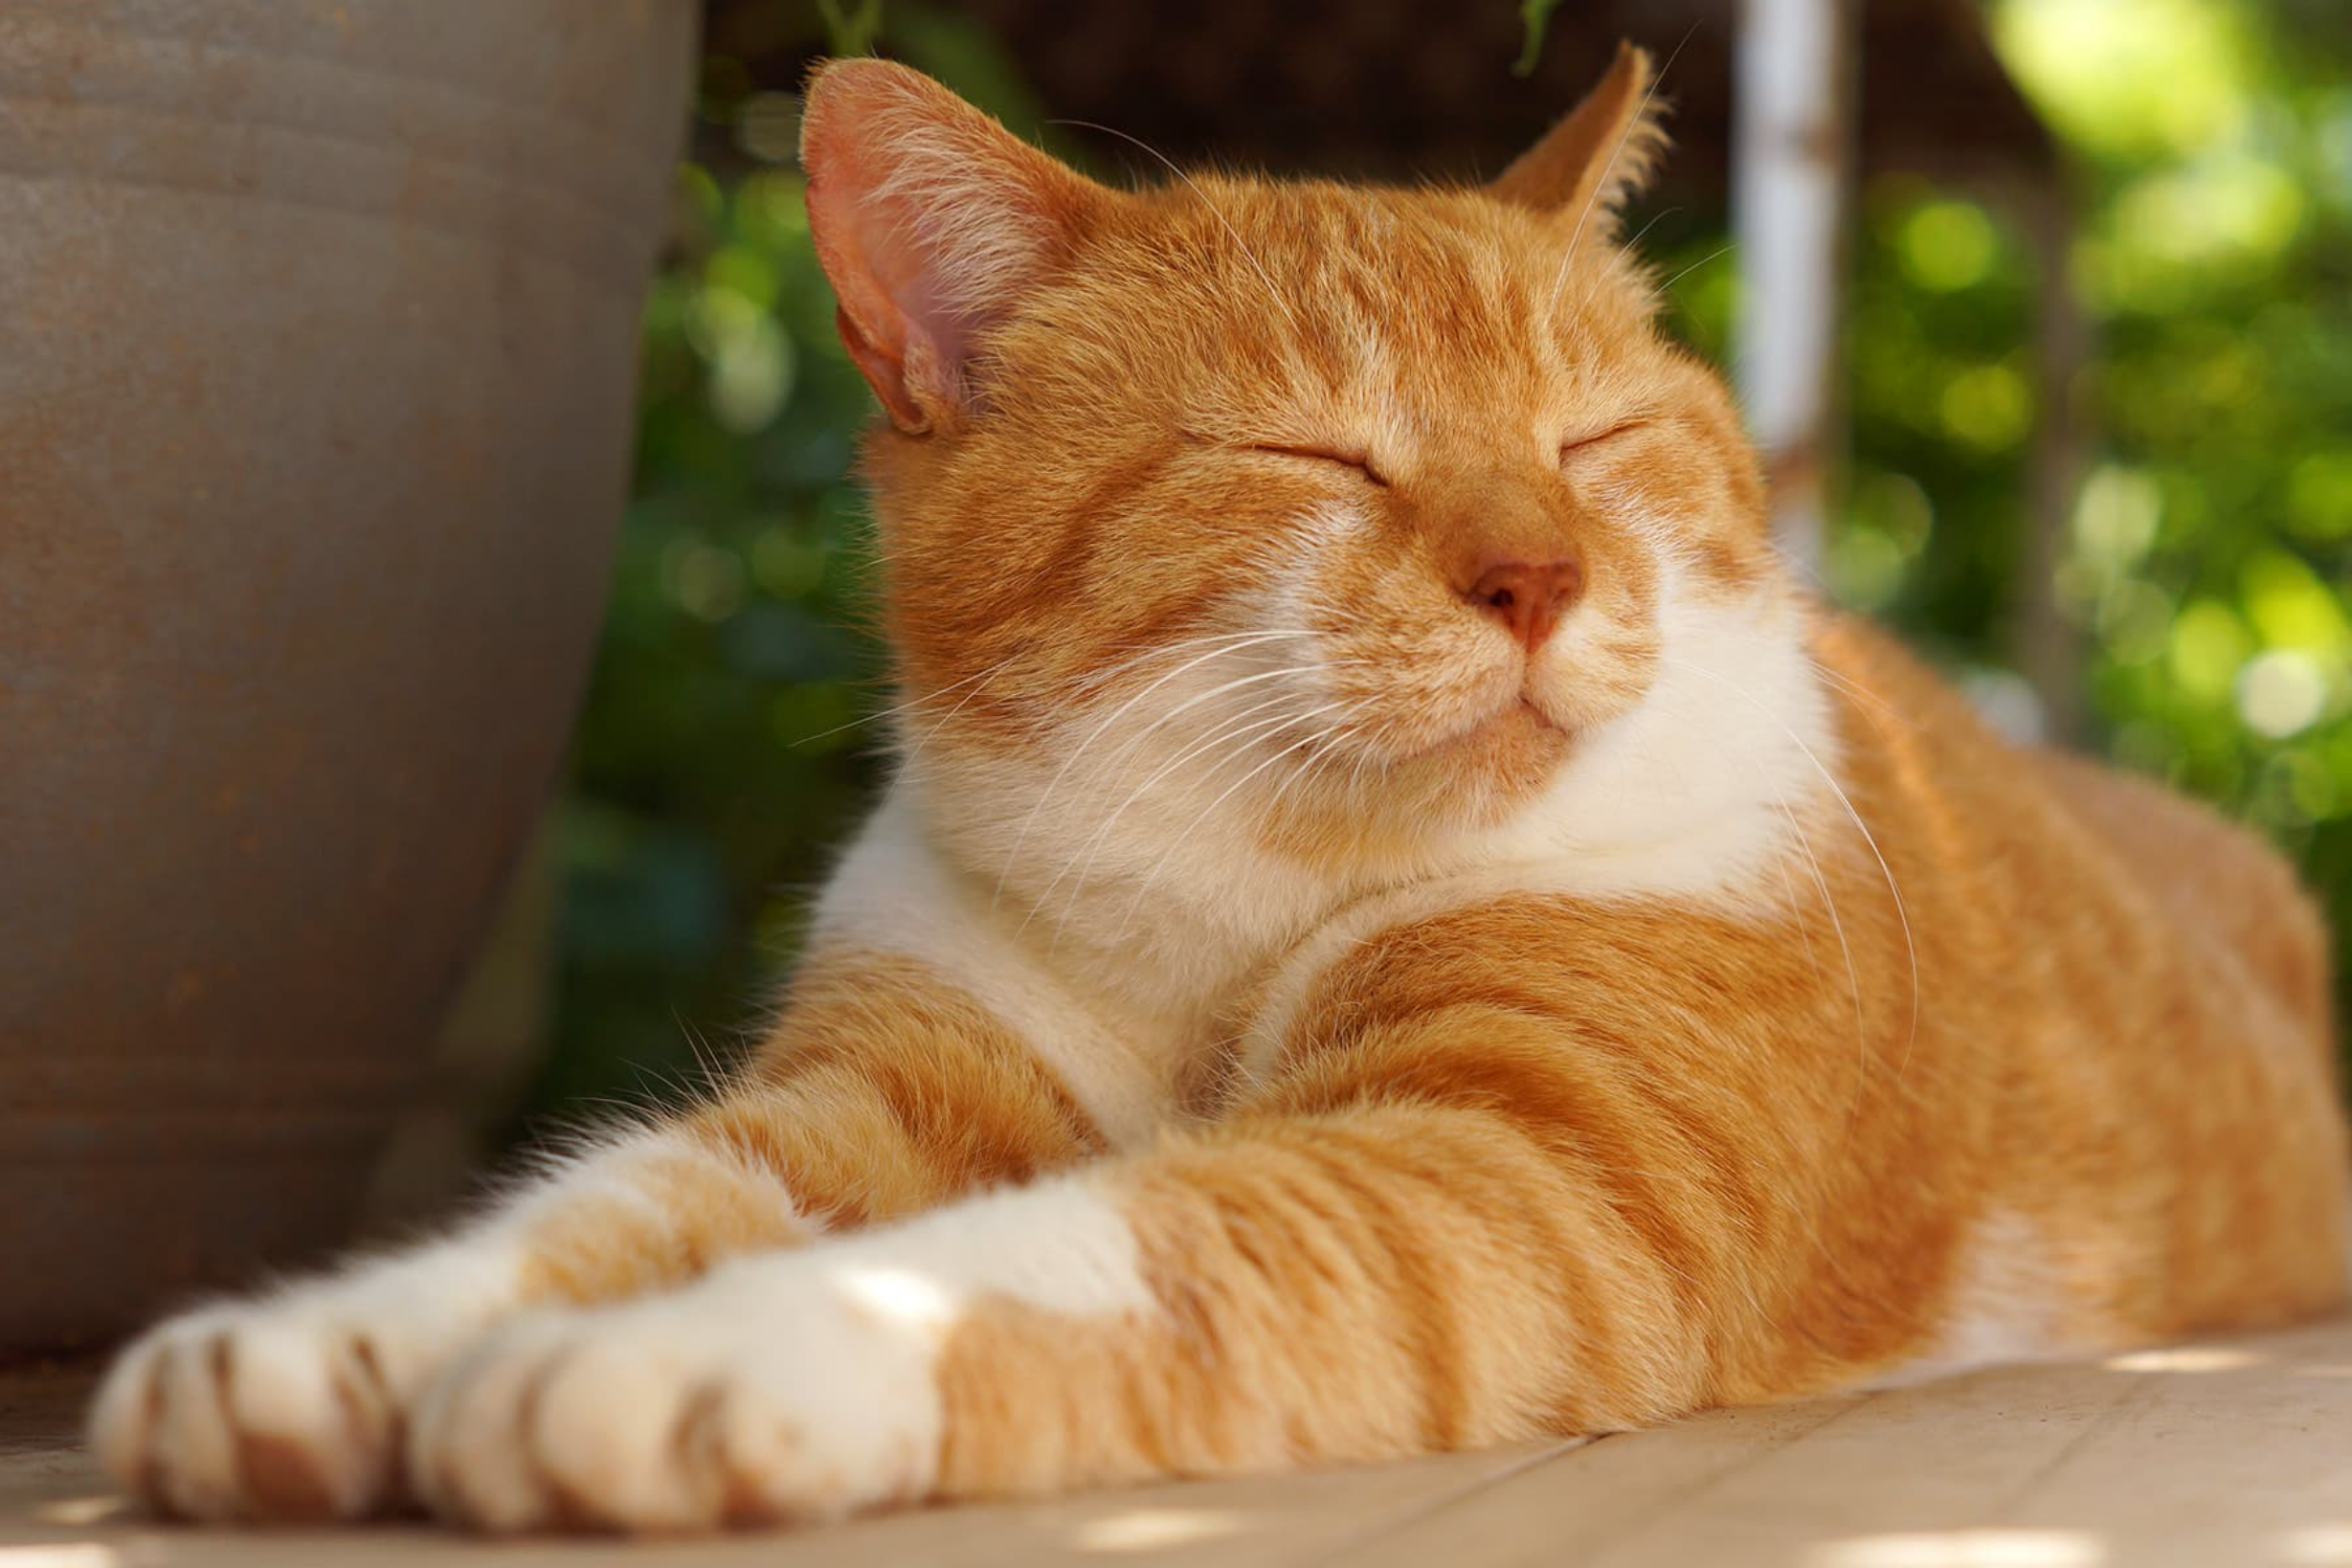
\includegraphics{cat_wide.png}
            \caption[Example of a much wider image]{I recommend making use of the landscape package in order to rotate pages and accommodate larger images and tables. Recommended width for landscape images is approximately 205mm. The afterpage package can help in placing landscape figures and tables without disrupting the flow of text on the page. Feel free to google the documentation on both packages to learn how to use them.}
        \label{fig:cats_wide}
    \end{figure} 
\end{landscape}}

Esse Lorem ad amet anim eu officia aliquip est. Et voluptate nulla aliquip irure exercitation reprehenderit laboris nisi ut occaecat. Exercitation labore ipsum irure ipsum elit qui eu esse.
Adipisicing fugiat aliqua labore excepteur labore labore Lorem officia officia nostrud excepteur eu nulla. Deserunt culpa veniam nulla qui ut incididunt consequat fugiat sint consectetur minim. Ea officia commodo consectetur voluptate cillum irure pariatur duis duis minim laborum cillum excepteur ex.

Sint do laboris magna officia ad occaecat cupidatat velit veniam ut nulla ullamco duis sit. Commodo excepteur reprehenderit in velit nulla cillum. Incididunt sunt laboris veniam officia. Dolor dolor ullamco et minim in ad veniam fugiat. Qui elit commodo eiusmod ea amet pariatur sit minim sit consequat culpa magna. Magna nulla non nulla ullamco do exercitation.
Ad velit ipsum laboris tempor pariatur non dolor exercitation mollit occaecat eu et. Ex commodo et tempor id in in amet occaecat pariatur excepteur proident do. Elit incididunt laborum ullamco cupidatat ut dolor elit velit est tempor dolor aliquip. In velit exercitation nostrud qui fugiat nostrud labore dolore proident proident labore sint quis ipsum. Dolore nostrud commodo quis sint commodo ea deserunt. Tempor officia proident anim fugiat aute nostrud exercitation deserunt sunt.

Sit deserunt ex aliquip reprehenderit minim incididunt adipisicing officia reprehenderit enim. Culpa eu occaecat cillum Lorem ex ad id minim adipisicing laborum velit nulla ea. Tempor sunt ut sint consectetur minim magna tempor labore cupidatat consectetur. Dolor sit ut magna incididunt commodo dolore nulla mollit ullamco id sunt irure anim enim.
Aliqua duis id aute esse consectetur fugiat elit cillum commodo non reprehenderit. Proident reprehenderit velit dolor laboris ipsum magna nulla laborum cupidatat anim esse voluptate deserunt. Magna amet sint elit est elit. Ad esse incididunt tempor amet labore quis. Cupidatat sit minim officia consectetur.

\section{Conclusions}
Elit nulla anim aliqua sunt et ex duis pariatur adipisicing esse elit duis tempor ea. Elit Lorem consectetur duis occaecat minim proident deserunt amet. Veniam irure commodo aute do adipisicing qui deserunt velit quis dolor exercitation. Deserunt excepteur exercitation esse exercitation sint magna reprehenderit. Magna enim duis nulla dolore aute commodo ullamco consectetur anim nulla adipisicing labore laborum cillum. Ex veniam esse consequat officia laborum aliqua laboris ullamco ad esse sint mollit.

Ex proident enim excepteur deserunt in sit. Lorem dolore adipisicing consequat laborum ut et dolor minim ullamco sit mollit. Enim reprehenderit exercitation laboris deserunt sint minim exercitation qui ea. Pariatur sunt ad in esse exercitation eu incididunt labore esse exercitation aute laborum qui. Magna aliqua do do nostrud voluptate qui reprehenderit magna.
Exercitation sit commodo duis laboris ea id excepteur cupidatat anim velit occaecat tempor. Elit aliqua enim laboris qui dolor cupidatat laboris quis qui. Excepteur deserunt qui sit ullamco sunt et anim aliqua sit commodo. Est proident id ex et nisi nostrud id qui culpa consequat sunt commodo. Cillum officia excepteur duis esse ea voluptate.

Ipsum esse aliquip consequat incididunt fugiat. Laboris fugiat reprehenderit do labore incididunt sunt eu in ipsum exercitation nulla velit dolore officia. Sunt veniam quis do occaecat qui cupidatat non sunt est reprehenderit consectetur.

\section{Acknowledgements}
I would never have made it this far without my dog, Mr Snuffelupagus.











\published{statement_of_authorship.JPG}
\chapter{The second of hopefully not too many chapters \label{ch:numero_dos}}
\begin{abstract}

This chapter has been published and therefore requires a \textbf{statement of authorship}! This package contains a \textbackslash published\{\} command that will include an image of a (preferably) signed statement of authorship and fit it to the margins of the page. It uses the \textbackslash includegraphics command behind the scenes so you should link to a file that is contained in one of your graphics path folders. I recommend cropping your form to remove whitespace and saving as an image file. This will fit the form nicely in the margins of the thesis document. I'm sure there is a more elegant way to handle this but it's not something I could be bothered working out!

Sit tempor ipsum consequat ea. Nisi exercitation culpa cupidatat excepteur proident mollit. Veniam cupidatat esse Lorem laboris veniam consectetur minim ex sint nostrud. Deserunt pariatur tempor exercitation consectetur tempor cillum elit labore velit consequat officia aliquip id dolore.
Eu pariatur enim dolore esse magna consectetur fugiat. Dolor incididunt elit amet laborum nulla consequat deserunt ex qui cillum. Ut anim cupidatat Lorem aliquip nulla dolor ullamco cupidatat ea nostrud velit pariatur Lorem. Est quis incididunt non eiusmod magna fugiat magna veniam labore irure qui. Non consectetur nulla cupidatat laborum mollit id.

Aliqua ullamco ea eu excepteur duis cillum aliquip do in sit ullamco ea est. Lorem reprehenderit voluptate mollit in dolore id occaecat labore. Est voluptate proident cillum ipsum deserunt tempor in. Incididunt proident deserunt sunt labore minim amet sint. Qui cillum non et dolor minim nulla aute nisi Lorem irure.
Aliqua ullamco ea eu excepteur duis cillum aliquip do in sit ullamco ea est. Lorem reprehenderit voluptate mollit in dolore id occaecat labore. Est voluptate proident cillum ipsum deserunt tempor in. Incididunt proident deserunt sunt labore minim amet sint. Qui cillum non et dolor minim nulla aute nisi Lorem irure.
\end{abstract}

\section{Introduction}
Dolor non officia anim ut dolor anim duis elit ullamco aliquip magna cupidatat. Magna ea ipsum enim laboris labore duis cillum commodo minim. Id anim sint ad et do deserunt ea esse.

Minim sint duis sunt adipisicing ad. Occaecat labore in eu ad dolor adipisicing consequat. Do occaecat Lorem consectetur quis aliquip dolore consequat aliquip proident voluptate est ipsum cillum. Dolor ea veniam adipisicing veniam do ut laborum consequat laboris reprehenderit aliquip. Excepteur Lorem dolore amet esse dolor duis adipisicing quis dolore laboris cillum voluptate. In mollit aliquip duis do aute.

Culpa eiusmod irure occaecat sint commodo pariatur nostrud anim id velit pariatur. Eiusmod dolore consequat sint enim dolor aliquip minim sit ullamco non occaecat occaecat. Fugiat exercitation nostrud culpa occaecat fugiat adipisicing enim ut occaecat mollit non pariatur. Sint dolor aliquip velit eu do cupidatat quis. Culpa sint velit ex esse ex.

Fugiat amet sit cillum duis. Eiusmod nisi nulla cillum laborum labore non. Officia incididunt ea elit tempor excepteur mollit eiusmod Lorem ullamco. Do cupidatat sunt nisi pariatur proident enim adipisicing pariatur officia incididunt sunt nostrud reprehenderit in. Est amet excepteur ad laborum cillum laboris Lorem officia id. Voluptate velit aute Lorem ea eiusmod veniam.

Ut laboris aute tempor duis ad irure minim ea pariatur eu est tempor mollit anim. Nulla voluptate voluptate nostrud minim exercitation ex qui excepteur sint amet in veniam. Est minim aliquip consequat aliquip aute ullamco enim et aliquip. Aliquip sunt do aute reprehenderit ullamco occaecat consequat non. Ipsum nostrud in culpa adipisicing consectetur eu ad dolore in sint est id.

\section{Background}
Aliquip voluptate enim anim sunt occaecat nisi quis tempor sint Lorem do dolor magna aliqua. Magna voluptate non esse qui nostrud est laborum cupidatat aliquip officia nisi. Officia in veniam id deserunt tempor elit pariatur aute amet ea labore. Minim cillum commodo do aute et ut commodo aliqua sit in. Pariatur ut commodo quis culpa mollit sint Lorem. Nisi velit velit do non commodo reprehenderit aute dolore ullamco ea qui.
Laboris eiusmod velit reprehenderit aliqua eu laboris ea Lorem occaecat ad et anim officia. In pariatur non ullamco consequat sint elit ullamco consectetur aute anim incididunt qui. Et exercitation ad mollit amet. Ipsum esse nisi aliquip duis excepteur. Laboris esse deserunt voluptate nulla laboris exercitation aliqua.




Nisi ad eu et est magna mollit consequat dolor irure quis commodo ex laborum nostrud. Aliquip non nisi occaecat Lorem quis aliquip quis reprehenderit veniam nisi ad elit mollit. Ut quis quis exercitation enim pariatur ut ut sint tempor labore velit id. Aute veniam ex commodo non laboris. Est occaecat excepteur do excepteur ipsum ad quis.
Et exercitation cupidatat cillum nostrud sit do aliqua quis officia ullamco ullamco aute sunt laboris. Laborum officia do pariatur consectetur ut cillum ut id pariatur excepteur exercitation pariatur laboris consectetur. Aliqua cillum id minim commodo nulla Lorem enim nostrud.

Est commodo laboris ea voluptate consectetur aliqua. Nostrud officia magna proident voluptate labore consequat. Esse tempor est est aliqua dolor sunt sit ea sint. Culpa ipsum cillum enim ipsum in cillum esse consectetur. Nulla mollit sunt sint laborum consectetur commodo reprehenderit cupidatat tempor do minim laborum elit anim. Sit id nisi consequat ipsum nostrud reprehenderit ea voluptate deserunt nulla velit nostrud esse.
Ullamco nisi consequat pariatur nisi dolore cupidatat voluptate voluptate sit velit. Velit sit nulla incididunt est ea nulla. Laboris mollit culpa mollit magna reprehenderit adipisicing ut elit deserunt dolore. Quis consectetur incididunt minim exercitation voluptate veniam. Ut irure fugiat quis eiusmod. Voluptate non quis amet incididunt ipsum. Nostrud officia ut commodo incididunt fugiat reprehenderit sunt enim consectetur qui.

Eu enim ut nulla irure pariatur consequat do id excepteur cillum eiusmod sit culpa aliqua. Amet magna mollit tempor elit minim duis laborum cupidatat consequat quis. Magna deserunt esse veniam consequat cupidatat irure ea nulla sunt est aliqua eu aliqua officia. Anim in proident esse voluptate. Deserunt in tempor amet reprehenderit officia exercitation nulla eu nisi qui commodo ullamco ea.
Ea do excepteur laboris exercitation aliquip et. Cupidatat nulla eiusmod incididunt magna labore ea incididunt tempor mollit incididunt. Nisi cupidatat sint incididunt aliquip excepteur pariatur velit in tempor est sint. Culpa cupidatat velit anim dolore irure.

Commodo aliqua non reprehenderit nulla quis culpa incididunt laboris nisi eiusmod. Laboris eu ut et minim sunt excepteur esse eiusmod amet veniam labore do. Consectetur sunt incididunt ipsum tempor eu. Id labore veniam ut nisi non aliqua occaecat eu eiusmod non fugiat sint. Duis velit fugiat nisi esse nostrud laborum.
Sint non irure mollit excepteur amet aliquip excepteur et mollit id in. Ut ad voluptate deserunt ut. Ex culpa nostrud exercitation pariatur aliqua.

\section{Methods}
Magna dolore laboris magna et commodo. Ut aliqua veniam officia do in officia consequat proident eu labore esse aliquip mollit. Veniam elit qui nisi amet est sit anim. Labore pariatur excepteur cillum irure quis. Est minim ad culpa commodo est sint excepteur irure labore ex.
Ea id ullamco quis est sunt officia duis. Voluptate ex laborum nostrud minim non fugiat enim. Et velit in culpa et sunt est anim excepteur eiusmod esse. Eu culpa amet aliqua aliquip dolor officia et veniam commodo.
Eu occaecat laboris voluptate aliqua. Esse Lorem amet occaecat aute adipisicing commodo labore non quis est esse. Nulla deserunt consequat officia cupidatat irure minim amet eu velit est ex ex. Ipsum ipsum dolore consequat veniam cillum sit irure. Ipsum deserunt in laboris tempor non laboris est. In enim officia occaecat magna ad est est esse Lorem officia Lorem minim laboris.

Irure nisi elit qui elit id fugiat consectetur deserunt. Ullamco nostrud cillum esse nisi sunt. Proident commodo minim aliquip amet adipisicing amet cupidatat mollit incididunt nisi do excepteur proident voluptate. Duis incididunt exercitation in veniam irure labore reprehenderit sint occaecat et non.
Reprehenderit mollit veniam laboris labore eu consectetur labore culpa dolor magna ex deserunt. Sit eiusmod et duis veniam nulla do veniam eu enim ex eu minim id. Ut ex proident duis tempor et. Eiusmod dolor occaecat sint ipsum officia non pariatur enim tempor est eiusmod.

Id reprehenderit deserunt laborum mollit ullamco veniam laborum aute ad excepteur sit ullamco duis aliqua. Esse dolore do ex eu elit exercitation adipisicing deserunt irure. Et fugiat fugiat est nisi tempor quis. Dolore dolore officia do consectetur minim minim sunt officia culpa et ex.

\section{Results}
  
Irure nisi elit qui elit id fugiat consectetur deserunt. Ullamco nostrud cillum esse nisi sunt. Proident commodo minim aliquip amet adipisicing amet cupidatat mollit incididunt nisi do excepteur proident voluptate. Duis incididunt exercitation in veniam irure labore reprehenderit sint occaecat et non.
Reprehenderit mollit veniam laboris labore eu consectetur labore culpa dolor magna ex deserunt. Sit eiusmod et duis veniam nulla do veniam eu enim ex eu minim id. Ut ex proident duis tempor et. Eiusmod dolor occaecat sint ipsum officia non pariatur enim tempor est eiusmod.

\section{Discussion}
Occaecat do cillum enim aliqua elit qui nisi aliqua ullamco elit labore. Sit sunt adipisicing labore quis aute pariatur. Nulla reprehenderit ex laborum enim velit officia sint. Officia laborum velit ad fugiat cupidatat cillum consectetur dolor. Aute laborum incididunt dolore pariatur quis ad dolore deserunt elit Lorem velit esse dolore anim.
Laborum magna ea laborum qui cupidatat sint ex pariatur. Nulla laboris pariatur culpa minim est ut culpa fugiat amet exercitation nisi proident id anim. Labore elit voluptate minim labore mollit. Aliqua sit magna deserunt in id pariatur sint consectetur culpa anim labore amet in elit. Qui veniam id cupidatat anim aliqua dolore pariatur. Veniam laborum in excepteur laboris anim dolor pariatur ipsum id.

Ea commodo excepteur duis ea voluptate aliqua consequat et. Reprehenderit in dolore et dolor. Aliquip sunt do elit aliqua nisi Lorem sunt nostrud Lorem veniam irure incididunt ut ullamco. Fugiat enim aliqua consectetur sunt aute id dolore ad consequat adipisicing. Voluptate enim culpa pariatur dolor anim. In commodo officia enim proident est reprehenderit aute fugiat consequat dolore sit aute ad.
Cillum dolor sint laboris duis nisi sunt. In laboris veniam cillum cupidatat laboris laboris exercitation. Consectetur consequat nisi est ipsum duis incididunt ullamco elit sunt cupidatat anim exercitation proident eiusmod. Adipisicing reprehenderit incididunt commodo occaecat nostrud ipsum labore tempor sit nostrud occaecat dolor. Ullamco commodo Lorem labore nisi ullamco cupidatat mollit labore et officia enim. Incididunt ad voluptate cillum aliqua proident duis.

Esse Lorem ad amet anim eu officia aliquip est. Et voluptate nulla aliquip irure exercitation reprehenderit laboris nisi ut occaecat. Exercitation labore ipsum irure ipsum elit qui eu esse.
Adipisicing fugiat aliqua labore excepteur labore labore Lorem officia officia nostrud excepteur eu nulla. Deserunt culpa veniam nulla qui ut incididunt consequat fugiat sint consectetur minim. Ea officia commodo consectetur voluptate cillum irure pariatur duis duis minim laborum cillum excepteur ex.

Sint do laboris magna officia ad occaecat cupidatat velit veniam ut nulla ullamco duis sit. Commodo excepteur reprehenderit in velit nulla cillum. Incididunt sunt laboris veniam officia. Dolor dolor ullamco et minim in ad veniam fugiat. Qui elit commodo eiusmod ea amet pariatur sit minim sit consequat culpa magna. Magna nulla non nulla ullamco do exercitation.
Ad velit ipsum laboris tempor pariatur non dolor exercitation mollit occaecat eu et. Ex commodo et tempor id in in amet occaecat pariatur excepteur proident do. Elit incididunt laborum ullamco cupidatat ut dolor elit velit est tempor dolor aliquip. In velit exercitation nostrud qui fugiat nostrud labore dolore proident proident labore sint quis ipsum. Dolore nostrud commodo quis sint commodo ea deserunt. Tempor officia proident anim fugiat aute nostrud exercitation deserunt sunt.

Sit deserunt ex aliquip reprehenderit minim incididunt adipisicing officia reprehenderit enim. Culpa eu occaecat cillum Lorem ex ad id minim adipisicing laborum velit nulla ea. Tempor sunt ut sint consectetur minim magna tempor labore cupidatat consectetur. Dolor sit ut magna incididunt commodo dolore nulla mollit ullamco id sunt irure anim enim.
Aliqua duis id aute esse consectetur fugiat elit cillum commodo non reprehenderit. Proident reprehenderit velit dolor laboris ipsum magna nulla laborum cupidatat anim esse voluptate deserunt. Magna amet sint elit est elit. Ad esse incididunt tempor amet labore quis. Cupidatat sit minim officia consectetur.

\section{Conclusions}
Elit nulla anim aliqua sunt et ex duis pariatur adipisicing esse elit duis tempor ea. Elit Lorem consectetur duis occaecat minim proident deserunt amet. Veniam irure commodo aute do adipisicing qui deserunt velit quis dolor exercitation. Deserunt excepteur exercitation esse exercitation sint magna reprehenderit. Magna enim duis nulla dolore aute commodo ullamco consectetur anim nulla adipisicing labore laborum cillum. Ex veniam esse consequat officia laborum aliqua laboris ullamco ad esse sint mollit.

Ex proident enim excepteur deserunt in sit. Lorem dolore adipisicing consequat laborum ut et dolor minim ullamco sit mollit. Enim reprehenderit exercitation laboris deserunt sint minim exercitation qui ea. Pariatur sunt ad in esse exercitation eu incididunt labore esse exercitation aute laborum qui. Magna aliqua do do nostrud voluptate qui reprehenderit magna.
Exercitation sit commodo duis laboris ea id excepteur cupidatat anim velit occaecat tempor. Elit aliqua enim laboris qui dolor cupidatat laboris quis qui. Excepteur deserunt qui sit ullamco sunt et anim aliqua sit commodo. Est proident id ex et nisi nostrud id qui culpa consequat sunt commodo. Cillum officia excepteur duis esse ea voluptate.

Ipsum esse aliquip consequat incididunt fugiat. Laboris fugiat reprehenderit do labore incididunt sunt eu in ipsum exercitation nulla velit dolore officia. Sunt veniam quis do occaecat qui cupidatat non sunt est reprehenderit consectetur.

\section{Acknowledgements}
Ipsum esse aliquip consequat incididunt fugiat. Laboris fugiat reprehenderit do labore incididunt sunt eu in ipsum exercitation nulla velit dolore officia. Sunt veniam quis do occaecat qui cupidatat non sunt est reprehenderit consectetur.












% continue with as many chapter as required
\conclusions
Reprehenderit voluptate fugiat qui mollit nulla occaecat officia consectetur non voluptate culpa cillum tempor aliqua. Laborum tempor mollit excepteur laboris. Laboris sint et in exercitation nostrud laboris ipsum eiusmod. Fugiat incididunt eiusmod incididunt Lorem. Ipsum cillum Lorem aliqua ex occaecat occaecat ex elit veniam tempor. Reprehenderit duis esse enim aute officia.
Ut culpa reprehenderit proident nostrud qui anim duis cillum eu incididunt. Voluptate aliqua in aliquip pariatur amet do consectetur. Incididunt proident sunt eu officia do ex qui ea mollit. Esse et excepteur incididunt enim excepteur do ullamco sit proident officia aliquip. Mollit eu ipsum ex quis est esse id deserunt est. Amet occaecat tempor dolor sit nulla. Veniam quis elit Lorem aliqua consectetur consequat occaecat.

Ea cillum mollit ut tempor consectetur ea consectetur. Magna quis in consequat labore do labore officia incididunt Lorem eu. Minim tempor officia consequat veniam. Ex anim et officia voluptate enim aliquip ad ad veniam mollit fugiat tempor est. Sint pariatur consequat Lorem incididunt duis reprehenderit esse exercitation cillum est id eu cupidatat. Exercitation voluptate cillum cupidatat veniam adipisicing incididunt sit et adipisicing magna deserunt tempor.
Cupidatat ipsum dolore quis nisi. Culpa duis in nisi quis ex enim aliquip fugiat cillum. Labore magna dolore esse in non aliquip exercitation labore aliquip eu velit dolor quis. Nisi sit in quis quis labore.

Commodo ea esse non commodo pariatur duis ut culpa laborum. Reprehenderit excepteur consequat aliqua eu nulla esse in ex voluptate nulla. Tempor incididunt laborum anim dolor deserunt occaecat.
Consequat pariatur nostrud do id voluptate incididunt sunt sint sunt ad. Esse Lorem minim in et fugiat dolor. Nostrud ad est cupidatat cillum. Officia ut occaecat fugiat adipisicing do.
Id cupidatat in est laborum eiusmod minim. Dolore qui magna dolor irure proident proident eiusmod ex laboris enim aliqua. Velit laboris et quis velit ea ullamco duis cillum velit eiusmod irure non eu sit. Incididunt enim aute labore pariatur sint. Cupidatat sunt consequat voluptate fugiat consectetur minim esse. Fugiat elit eiusmod laborum consectetur velit anim officia proident.

Et excepteur sint amet occaecat qui dolor. Tempor deserunt dolore id magna consequat laborum sunt. Qui culpa est id laborum eu deserunt dolor incididunt non eiusmod et est ex. Id anim commodo nostrud tempor fugiat cillum ex culpa eu dolore in laborum veniam. Excepteur adipisicing exercitation deserunt nulla deserunt amet officia tempor incididunt cillum qui. Fugiat quis ut incididunt enim labore dolor. In ut sunt deserunt ullamco nostrud irure eiusmod adipisicing sunt magna consequat.
Fugiat sunt commodo nostrud veniam dolore id. Tempor ut Lorem enim ullamco mollit magna. Labore Lorem ipsum minim incididunt tempor velit ea mollit exercitation aliquip pariatur ea. Ipsum voluptate quis adipisicing ut non dolor.

Reprehenderit ipsum tempor labore duis tempor culpa duis non anim amet id reprehenderit aliquip. Dolore et in non aliqua. Qui ut est magna sit sit in proident et aliqua elit sint voluptate eiusmod esse. Cillum anim ea eu ullamco culpa dolore eiusmod incididunt esse.

\appendix
\cleardoublepage
% Import the appendices 
\chapter{My appendices from chapter 1 \label{app:chapter_1}}
% I like to do a seperate appendix file for each chapter and save it in the appropriate folder

\section{First appendix section}
Minim sint duis sunt adipisicing ad. Occaecat labore in eu ad dolor adipisicing consequat. Do occaecat Lorem consectetur quis aliquip dolore consequat aliquip proident voluptate est ipsum cillum. Dolor ea veniam adipisicing veniam do ut laborum consequat laboris reprehenderit aliquip. Excepteur Lorem dolore amet esse dolor duis adipisicing quis dolore laboris cillum voluptate. In mollit aliquip duis do aute.

\section{Second appendix section if required}
Fugiat amet sit cillum duis. Eiusmod nisi nulla cillum laborum labore non. Officia incididunt ea elit tempor excepteur mollit eiusmod Lorem ullamco. Do cupidatat sunt nisi pariatur proident enim adipisicing pariatur officia incididunt sunt nostrud reprehenderit in. Est amet excepteur ad laborum cillum laboris Lorem officia id. Voluptate velit aute Lorem ea eiusmod veniam.

Ut laboris aute tempor duis ad irure minim ea pariatur eu est tempor mollit anim. Nulla voluptate voluptate nostrud minim exercitation ex qui excepteur sint amet in veniam. Est minim aliquip consequat aliquip aute ullamco enim et aliquip. Aliquip sunt do aute reprehenderit ullamco occaecat consequat non. Ipsum nostrud in culpa adipisicing consectetur eu ad dolore in sint est id. 

\backmatter
% Add the bibliography to the table of contents
\addcontentsline{toc}{chapter}{Bibliography}
\bibliographystyle{apa} % choose whatever style you wish, I don't believe there is a requirement from the university
\bibliography{reference_list}


\end{document}

